% ============================================================================
% Accessibility
% ============================================================================
\DocumentMetadata{
  lang = en-US, 
  pdfstandard = ua-2, 
  tagging = on, 
  tagging-setup = {math/setup=mathml-SE}
}

% ============================================================================
% Document Properties - used on title slide and PDF metadata fields
% ============================================================================
\def\PresTitle{Line Measurement}  % Required - top line of title slide
\def\PresSubtitle{Baker College Engineering}         % Optional - second line
\def\PresAuthor{Brad Peirson}               % Required - below dividing line
\def\PresInstitute{College of Information Technology and Engineering}       % Optional
\def\PresDate{}                             % Optional
\def\PresKeywords{}                         % Optional - used for hyperref

% Presentation Formatting
% ============================================================================
% ============================================================================
% Class Declaration
% ============================================================================
\documentclass[
        mode = handout,     % Projector = one bullet at a time, Handout = all
        font-size=14pt,     % Only accepts 9, 10, 12, 14, 17, 20
        pdfusetitle         % Pulls \title property from document
    ]
    {ltx-talk}              % ltx-talk class

% ============================================================================
% Custom Colors
% ============================================================================
\usepackage[table]{xcolor}
% Colors from the Baker College Style Guide
%\definecolor{BakerADARed}{RGB}{231, 0, 46}   % #e7002e Official ADA red-doesn't pass WCAG AAA for small text
\definecolor{BakerADARed}{RGB}{181, 0, 36}    % #b50024 Adjusted ADA red-passes WCAG AAA for small text
\definecolor{HoneyYellow}{RGB}{255, 196, 0}   % #ffc400
\definecolor{UpNorthGreen}{RGB}{114, 191, 68} % #72bf44
\definecolor{LakeBlue}{RGB}{134, 183, 227}    % #86b7e3
\definecolor{BakerADI}{RGB}{58, 98, 170}
\definecolor{BakerCIM}{RGB}{217, 35, 47}
\definecolor{BakerBlack}{RGB}{31, 34, 40}     % #1f2228
\definecolor{BakerWhite}{RGB}{255, 255, 255}
\definecolor{BakerRed}{RGB}{239, 0, 48}
\definecolor{Abbey}{RGB}{80, 82, 88}
\definecolor{RollingStone}{RGB}{121, 124, 126}
\definecolor{HitGray}{RGB}{165, 169, 172}
\definecolor{Iron1}{RGB}{201, 206, 209}
\definecolor{Iron}{RGB}{222, 225, 226}
\definecolor{BlackHaze1}{RGB}{237, 240, 240}
\definecolor{BlackHaze}{RGB}{245, 247, 247}

% ============================================================================
% Document Data
% ============================================================================
\title{\PresTitle}
\author{\PresAuthor}
\institute{\PresInstitute}
\date{\PresDate}

%Set up the hyperlink colors
\hypersetup{colorlinks,
    linkcolor=BakerBlack,
    urlcolor=BakerADARed,
    pdfauthor = {\PresAuthor},
    %pdftitle = {\PresentationTopic},   % Title is pulled directly
    pdfsubject = {\PresSubtitle},
    pdfkeywords = {\Keywords},
    pdfcreator = {LaTeX with hyperref package},
    pdfproducer = {LuaLaTeX}
    }

% Map your custom style guide colors to the progress bar aliases
\colorlet{pbcomplete}{BakerADARed}
\colorlet{pbincomplete}{Iron}

\usepackage[most]{tcolorbox}

% ============================================================================
% Footer Format
% ============================================================================
\EditInstance{footer}{std}{
  color         = Abbey,
  separator     = \hfill,
  element-order = {title, institute, framenumber},
  right-hspace  = 3mm,
  left-hspace   = 3mm,
}

% \DeclareInstance{footer}{empty}{
%   element-order = {}
% }

% ============================================================================
% Progress Bar Toggles & Helper Macros
% ============================================================================
\usepackage{xfp}        % Needed for floating point math
\newif\ifprogressbar    % Used to determine whether or not to show the bar
\progressbartrue        % Set the bar to true at the start

% Helper macro to automatically turn off the progress bar inside title/section frames
\newcommand{\makeblindframe}[1]{%
  \progressbarfalse
  #1%
  \progressbartrue
}

% ============================================================================
% Custom Page Formats
% ============================================================================
\let\oldmaketitle\maketitle         % Backup the original maketitle command
\let\oldsection\section             % Backup the original section command
\let\oldsubsection\subsection       % Backup the original subsection command

\makeatletter
\renewcommand{\maketitle}{%
\makeblindframe{%
  \disableglobalbackground
  \slidebackground{PresentationTitleGraphic_2048x1151}%
  \color{white}%
  %\UseInstance{footer}{wallpaper}
  \begin{frame}[wallpaper]
    \vspace*{1in}%
      \begin{tcolorbox}[
          enhanced,
          colback=black,       
          colframe=black,      
          opacityfill=0.25,       
          arc=6pt,                
          boxrule=0pt,            
          left=20pt, right=20pt,  
          top=20pt, bottom=20pt,
          width=0.80\textwidth,   
          halign=left             
      ]
          \color{white}%
          % Title (Always visible)
          {\large\bfseries\sffamily \@title}\\[0.5em]%
          
          % Conditional Subtitle
          \ifx\PresSubtitle\empty
          \else
            {\normalsize\sffamily \PresSubtitle}\\[0.5em]%
          \fi
          
          % High-contrast divider line
          {\color{white!80}\rule{0.3\textwidth}{0.8pt}}\\[0.5em]%
          
          % Author (Always visible)
          {\small\sffamily \@author}\\%
          
          % Conditional Institute
          \ifx\PresInstitute\empty
          \else
            {\small\sffamily \PresInstitute}\\%
          \fi
          
          % Conditional Date
          \ifx\PresDate\empty
          \else
            {\small\sffamily \@date}\\%
          \fi
      \end{tcolorbox}%
      \vfill     
  \end{frame}%
  \enableglobalbackground{BG}%
  \color{black}%
  %\UseInstance{footer}{std}
}%
}
\makeatother

% Create a variable container to hold the current section title
\newcommand{\currentsectiontitle}{}

% Redefine \section to take 1 argument (the title)
\renewcommand{\section}[1]{%
\makeblindframe{%
  \renewcommand{\currentsectiontitle}{#1}%
  \disableglobalbackground
  \slidebackground{PresentationSectionBackground_2048x1151}%
  \begin{frame}
    \vfill
    %\vspace*{0.625in}%
    \begin{tcolorbox}[
        enhanced,
        colback=black,       
        colframe=black,      
        opacityfill=0.25,       
        arc=6pt,                
        boxrule=0pt,            
        left=20pt, right=20pt,  
        top=20pt, bottom=20pt,
        width=0.80\textwidth,   
        halign=left             
    ]
        \color{white}%
        {\large\bfseries\sffamily #1}\\[0.5em]%   
    \end{tcolorbox}%
    \vfill 
  \end{frame}%
  \oldsection{#1}%
  \enableglobalbackground{BG}%

  % This will be used for an auto TOC at every section
  % Right now ltx-talk TOC is still in development
  % Once it comes a little further along this can be used
  % \begin{frame}
  %       \frametitle{Section Overview}
  %       \tableofcontents[sections=\thesection]
  %   \end{frame}%
}%
}

% Redefine \subsection to take 1 argument
\renewcommand{\subsection}[1]{%
\makeblindframe{%
  \disableglobalbackground
  \slidebackground{PresentationSectionBackground_2048x1151}%
  \begin{frame}
    \vfill
    %\vspace*{0.25in}% 
    \begin{tcolorbox}[
        enhanced,
        colback=black,       
        colframe=black,      
        opacityfill=0.25,       
        arc=6pt,                
        boxrule=0pt,            
        left=20pt, right=20pt,  
        top=20pt, bottom=20pt,
        width=0.80\textwidth,   
        halign=left             
    ]
        \color{white}%
        {\large\bfseries\sffamily\currentsectiontitle}\\[0.5em]%
        {\normalsize\sffamily #1}%
    \end{tcolorbox}%
    \vfill 
  \end{frame}%
  \oldsubsection{#1}%
  \enableglobalbackground{BG}%
}%
}

%Set the fonts to use NeueHaas Grotesk
\setsansfont{NHAASGROTESKTXPRO-}[
    Path=../NeueHaasGroteskFiles/,
    Scale=1.0,
    Extension = .ttf,
    UprightFont=*55Rg,
    BoldFont=*75Bd,
    ItalicFont=*56It,
    BoldItalicFont=*76BdIt
    ]

% Force the document default family to Sans-Serif
\renewcommand{\familydefault}{\sfdefault}

\usepackage{mathtools} % Load BEFORE unicode math settings
\setmathfont{Fira Math}[Scale=MatchLowercase] 

% 1. Turn global background ON
\newcommand{\enableglobalbackground}[1]{%
  \AddToHook{shipout/background}[mybg]{%
    \put(0, -\paperheight){%
      \includegraphics[width=\paperwidth, height=\paperheight, artifact]{#1}%
    }%
  }%
}

% 2. Turn global background OFF
\newcommand{\disableglobalbackground}{%
  \RemoveFromHook{shipout/background}[mybg]%
}

\newcommand{\slidebackground}[1]{%
  \AddToHookNext{shipout/background}{%
    \put(0, -\paperheight){%
      \includegraphics[width=\paperwidth, height=\paperheight, artifact]{#1}%
    }%
  }%
}

% --- GLOBAL BULLET OVERRIDES ---
\renewcommand{\labelitemi}{\color{BakerBlack}\Large\textbullet}
\renewcommand{\labelitemii}{\color{BakerBlack}\large\textbullet}
\renewcommand{\labelenumi}{\color{BakerBlack}\bfseries\arabic{enumi}.}
\renewcommand{\labelenumii}{\color{BakerBlack}\bfseries\alph{enumii})}

\AddToHook{begindocument/before}{%
  \EditInstance{item}{description}{
    label-format = \normalfont\bfseries\color{BakerADARed}#1
  }%
}

\AddToHook{begindocument/before}{%
  \EditInstance{item}{basic}{
    label-format = \color{BakerADARed}#1
  }%
}

% Global override for ltx-talk slide titles
\EditInstance{frametitle}{header}{
    font = \rule{0pt}{1.5cm}\bfseries\Large,
}

\EditInstance{header}{std}{
    font = \bfseries\huge,
    color = BakerBlack,
}

\AddToHook{env/block/begin}{%
  \colorlet{structure}{BakerADARed}%
}

\pretocmd{\tableofcontents}{\begin{minipage}{\textwidth} \linespread{1.4}}{}{}
\apptocmd{\tableofcontents}{\end{minipage}}{}{}

%Biber not functional in ltx-talk as of 2026-05-29
%Package that allows the creation of bibliographies
\usepackage[
    backend=biber,
    style=authoryear,
    sorting=none,
    %entryhead=false
    ]{biblatex}

%Load the bibliography file
\addbibresource{../../reference.bib}

\defbibheading{bibslide}{References}

\newcolumntype{L}[1]{>{\raggedright\let\newline\\\arraybackslash\hspace{0pt}}m{#1}}
\newcolumntype{C}[1]{>{\centering\let\newline\\\arraybackslash\hspace{0pt}}m{#1}}
\newcolumntype{R}[1]{>{\raggedleft\let\newline\\\arraybackslash\hspace{0pt}}m{#1}}

%All of the graphics are in a seperate folder, this makes it so the folder doesn't have to be repeated every time
\graphicspath{
  {../assets/images}
  {../assets/diagrams}
  {../assets/plots}
}

\makeatletter
% New counter to hold the custom "max frames" for the progress bar
\newcommand{\pb@maxtotal}{1}

% Read the custom total from the .aux file if it exists
\AtBeginDocument{%
  \ifdefined\pb@storedtotal
    \let\pb@maxtotal\pb@storedtotal
  \else
    % Fallback to standard total if our custom hook hasn't run yet
    \edef\pb@maxtotal{\@totalframes}%
  \fi
}

% Custom Appendix command that caps the progress bar and turns it off
\newcommand{\talkappendix}{%
  % 1. Write the CURRENT frame number to the .aux file as the progress total
  \immediate\write\@auxout{\string\gdef\string\pb@storedtotal{\@framenumber}}%
  % 2. Turn off the progress bar for all subsequent appendix slides
  \progressbarfalse
}
\makeatother

% ============================================================================
% Progress Bar Logic 
% ============================================================================
\makeatletter               
\AddToHook{shipout/background}{%
  \ifprogressbar
    % Read ltx-talk's internal frame counter safely
    \edef\currentframe{\@framenumber}%
    \edef\totalframes{\pb@maxtotal}% Use our custom max total instead
    
    % Fallback checks: If the document hasn't fully compiled yet, default to 1
    \ifx\currentframe\empty\def\currentframe{1}\fi
    \ifx\totalframes\empty\def\totalframes{1}\fi
    
    % Draw the progress bar if we have a valid total frame count
    \ifnum\totalframes>1\relax
      % Compute fraction width: (current - 1) / (total - 1)
      \edef\pbfraction{\fpeval{(\currentframe - 1) / (\totalframes - 1)}}%
      
      % Guard rails to prevent the bar from overshooting 100% on a first compile
      \ifdim\pbfraction pt>1pt\def\pbfraction{1}\fi 
      
      \edef\completewidth{\fpeval{\pbfraction * \paperwidth}}%
      \edef\incompletewidth{\fpeval{\paperwidth - \completewidth}}%
      
      % Render full-width progress bar at the top edge
      \put(0cm, -0.1cm){%
        \color{pbcomplete}\rule{\completewidth pt}{2pt}%
        \color{pbincomplete}\rule{\incompletewidth pt}{2pt}%
      }%
    \fi
  \fi
}
\makeatother

% 1. Globally shrink all caption components right as the caption engine fires
\AddToHook{cmd/@makecaption/before}{\footnotesize}

% 2. Declare and assign a blank plug to the kernel's caption label socket
\NewSocketPlug{caption/label}{nolabel}{}
\AssignSocketPlug{caption/label}{nolabel}

\usepackage{adjustbox}

\usepackage{amssymb}
\usepackage{amsmath}

\usepackage{animate}

\usepackage{calc} % Optional, but helpful for layout

\usepackage{multirow}

\usepackage{textcomp}

\usepackage[americanvoltages]{circuitikz}
\usepackage{pgfplots}
\usepackage{pgf-pie}

\usetikzlibrary{
    intersections, 
    fillbetween,
    patterns,
    decorations.pathreplacing,
    decorations.pathmorphing,
    decorations.text,
    decorations.markings,
    arrows.meta,
    arrows,
    shapes,
    shapes.geometric,
    shadows,
    calligraphy,
    backgrounds,
    intersections,
    calc,
    math,
    positioning,
    svg.path,
    shadows,
    shadows.blur
    }

\pgfplotsset{compat=1.18}

\pgfdeclarelayer{ft}
\pgfdeclarelayer{bg}
\pgfsetlayers{bg, main, ft}

% Usage: \hexpic[]{height}{Alt text}{Attribution}{image path}
\newcommand{\hexpic}[5][]{%
  \begin{figure}
    \centering
    \begin{tikzpicture}[
      baseline=(hex.base),      
      every shadow/.style={
        shadow opacity=70
        }
      ]
      \node (hex) [
        draw=white, 
        minimum size=#2, 
        regular polygon, 
        regular polygon sides=6, 
        rotate=90,
        blur shadow
      ] {};
      \begin{scope}
        \clip (hex.corner 1) -- (hex.corner 2) -- (hex.corner 3) -- 
              (hex.corner 4) -- (hex.corner 5) -- (hex.corner 6) -- cycle;
        \node at (hex.center) [#1] {
          \includegraphics[height=#2, alt={#3}]{#5}
        };
      \end{scope}
    \end{tikzpicture}

    \vspace{0.5em}
    {\tiny #4\par}
  \end{figure}  
}

% Usage: \shadowpic[]{width}{Alt text}{Attribution}{image path}
\newcommand{\shadowpic}[5][]{%
  \begin{figure}
    \centering
    \begin{tikzpicture}
      [every shadow/.style={
        shadow opacity=70
        }
      ]
      \node (image) [
        inner sep=0,
        blur shadow
      ] {\includegraphics[width=#2, alt={#3}]{#5}};
    \end{tikzpicture}

    \vspace{0.5em}
    {\tiny #4\par}
  \end{figure}
}

\tikzset{middlearrow/.style={
        decoration={markings, 
        mark= at position 0.5 with {\arrow{#1}},
        },
        postaction={decorate}
    }
}

% Usage: \tikztodo[width]{height}{description/notes}
\newcommand{\tikztodo}[3][0.8\textwidth]{%
  \begin{center}
    \fbox{%
      \parbox[c][#2][c]{#1}{%
        \centering
        \textbf{\textcolor{red}{TODO: TikZ Diagram}}\\[0.5em]
        \small #3%
      }%
    }%
  \end{center}%
}

% Macro: \drawrails{<number_of_1cm_segments>}
\newcommand{\drawrails}[1]{
  % Calculate total depth: 1 cm per segment
  \pgfmathsetmacro{\railheight}{-1 * #1}
  
  % L1 Rail (x = 0)
  \draw[thick] (0, 0) -- (0, \railheight cm);
    
  % L2 Rail (x = 15)
  \draw[thick] (15, 0) -- (15, \railheight cm);
}

\newcommand{\ccwplus}{%
  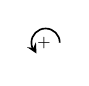
\begin{tikzpicture}[baseline=(char.base)]
    \node(char) at (0,0) {\(\scriptscriptstyle +\)};
    \draw[->, >=stealth, semithick] (0.2,0) arc (0:230:0.18cm);
  \end{tikzpicture}%
}

%====================================================================================
% Timer Ladder Symbol - Could be used for TON, TOF, RTO....
%====================================================================================
\tikzset{
    TON/.pic={

        \draw[
          BakerBlack
        ]
        (0,0)
        -- ++(0,0.375)
        -- ++(3.5,0)
        coordinate[pos=0.5](-TOP)
        -- ++(0,-1.75)
        coordinate[pos=3/14](-OUT)
        coordinate[pos=0.5](-EN1)
        coordinate[pos=0.875](-DN1)
        -- ++(-3.5,0)        
        -- (0,0)
        coordinate(-IN);

        \node[
          text=BakerBlack,
          font=\bfseries,
          anchor=east
        ](pre)
        at ($(-TOP)-(0,1.75em)$)
        {{\small PRE:}};

        \node[
          text=BakerBlack,
          font=\bfseries,
          anchor=east
        ](acc)
        at ($(pre.east)-(0,1em)$)
        {{\small ACC:}};

        \coordinate (-PRE) at (pre.east); % For the preset value
        \coordinate (-ACC) at (acc.east);

        \draw[
            BakerBlack
        ]
        (-EN1)
        -- ++(0.5,0)
        coordinate(-EN2)
        node[
            text=BakerBlack,
            anchor=west
        ]
        {{\small EN}};

        \draw[
            BakerBlack
        ]
        (-DN1)
        -- ++(0.5,0)
        coordinate(-DN2)
        node[
            text=BakerBlack,
            anchor=west
        ]
        {{\small DN}};

    }
}

%====================================================================================
% Oval ladder symbol, good for ONS, RES, etc.
%====================================================================================
\tikzset{
    ONS/.pic={

        \draw[
          BakerBlack
        ]
        (0,0)
        coordinate(-IN)
        -- ++(0.75,0)
        node[
          draw=BakerBlack, 
          text=BakerBlack, 
          font=\small, 
          minimum width=1.5cm, 
          minimum height=0.75cm, 
          anchor=west, 
          rounded corners=0.25cm
          ](ons){};
        
        \draw[BakerBlack] (ons.east) -- ++(0.75,0) coordinate(-OUT);

        \coordinate(-INS) at (ons.center);
        \coordinate(-VAR) at (ons.north); 
    }
}

%====================================================================================
% Source A, Source B, Dest box
%====================================================================================
\tikzset{
    SrcDest/.pic={
      
        \draw[
          BakerBlack
        ]
        (0,0)
        coordinate(-IN)
        -- ++(0,0.375)
        -- ++(5,0)
        coordinate[pos=0.5](-TOP)
        -- ++(0,-3.25)
        coordinate[pos=3/26](-OUT)
        -- ++(-5,0)
        -- (0,0)
        coordinate(l1);

        \node[
          text=BakerBlack,
          font=\bfseries,
          anchor=west
        ](srcA)
        at (l1)
        {{\small Src A:}};

        \node[
          text=BakerBlack,
          font=\bfseries,
          anchor=west
        ](srcB)
        at ($(l1)-(0,2em)$)
        {{\small Src B:}};

        \node[
          text=BakerBlack,
          font=\bfseries,
          anchor=west
        ](dest)
        at ($(srcB.west)-(0,2em)$)
        {{\small Dest:}};

        \coordinate(-SRCA) at (srcA.east);
        \coordinate(-AVAL) at ($(srcA.east)-(0,1em)$);
        \coordinate(-SRCB) at (srcB.east);
        \coordinate(-BVAL) at ($(srcB.east)-(0,1em)$);
        \coordinate(-DEST) at ($(-BVAL)-(0,1em)$);
        \coordinate(-DVAL) at ($(-DEST)-(0,1em)$);
    }
}

%====================================================================================
% Source A, Source B box
%====================================================================================
\tikzset{
    SrcAB/.pic={
      
        \draw[
          BakerBlack
        ]
        (0,0)
        coordinate(-IN)
        -- ++(0,0.375)
        -- ++(4,0)
        coordinate[pos=0.5](-TOP)
        -- ++(0,-2.25)
        coordinate[pos=1/6](-OUT)
        -- ++(-4,0)
        -- (0,0)
        coordinate(l1);

        \node[
          text=BakerBlack,
          font=\bfseries,
          anchor=west
        ](srcA)
        at (l1)
        {{\small Src A:}};

        \node[
          text=BakerBlack,
          font=\bfseries,
          anchor=west
        ](srcB)
        at ($(l1)-(0,2em)$)
        {{\small Src B:}};

        \coordinate(-SRCA) at (srcA.east);
        \coordinate(-AVAL) at ($(srcA.east)-(0,1em)$);
        \coordinate(-SRCB) at (srcB.east);
        \coordinate(-BVAL) at ($(srcB.east)-(0,1em)$);
    }
}

%====================================================================================
% LIMIT instruction
%====================================================================================
\tikzset{
    Limit/.pic={
      
        \draw[
          BakerBlack
        ]
        (0,0)
        coordinate(-IN)
        -- ++(0,0.375)
        -- ++(4,0)
        coordinate[pos=0.5](-TOP)
        -- ++(0,-3.25)
        coordinate[pos=3/26](-OUT)
        -- ++(-4,0)
        -- (0,0)
        coordinate(l1);

        \node[
          text=BakerBlack,
          font=\bfseries,
          anchor=west
        ](srcA)
        at (l1)
        {{\small Low:}};

        \node[
          text=BakerBlack,
          font=\bfseries,
          anchor=west
        ](srcB)
        at ($(l1)-(0,2em)$)
        {{\small Test:}};

        \node[
          text=BakerBlack,
          font=\bfseries,
          anchor=west
        ](dest)
        at ($(srcB.west)-(0,2em)$)
        {{\small High:}};

        \coordinate(-LO) at (srcA.east);
        \coordinate(-LOV) at ($(srcA.east)-(0,1em)$);
        \coordinate(-TEST) at (srcB.east);
        \coordinate(-TESTV) at ($(srcB.east)-(0,1em)$);
        \coordinate(-HI) at ($(-TESTV)-(0,1em)$);
        \coordinate(-HIV) at ($(-HI)-(0,1em)$);
    }
}

%====================================================================================
% Source Destination box
%====================================================================================
\tikzset{
    SrcSingle/.pic={
      
        \draw[
          BakerBlack
        ]
        (0,0)
        coordinate(-IN)
        -- ++(0,0.375)
        -- ++(6,0)
        coordinate[pos=0.5](-TOP)
        -- ++(0,-2.25)
        coordinate[pos=1/6](-OUT)
        -- ++(-6,0)
        -- (0,0)
        coordinate(l1);

        \node[
          text=BakerBlack,
          font=\bfseries,
          anchor=west
        ](srcA)
        at (l1)
        {{\small Source:}};

        \node[
          text=BakerBlack,
          font=\bfseries,
          anchor=east
        ](srcB)
        at ($(srcA.east)-(0,2em)$)
        {{\small Dest:}};

        \coordinate(-SRC) at (srcA.east);
        \coordinate(-SRCV) at ($(srcA.east)-(0,1em)$);
        \coordinate(-DEST) at (srcB.east);
        \coordinate(-DESTV) at ($(srcB.east)-(0,1em)$);
    }
}

%====================================================================================
% Compute Box
%====================================================================================
\tikzset{
    CPT/.pic={
      
        \draw[
          BakerBlack
        ]
        (0,0)
        coordinate(-IN)
        -- ++(0,0.375)
        -- ++(8.5,0)
        coordinate[pos=0.5](-TOP)
        -- ++(0,-1.75)
        coordinate[pos=3/14](-OUT)
        -- ++(-8.5,0)
        -- (0,0)
        coordinate(l1);

        \node[
          text=BakerBlack,
          font=\bfseries,
          anchor=west
        ](srcA)
        at (l1)
        {{\small Source:}};

        \node[
          text=BakerBlack,
          font=\bfseries,
          anchor=east
        ](srcB)
        at ($(srcA.east)-(0,2em)$)
        {{\small Exp:}};

        \coordinate(-DEST) at (srcA.east);
        \coordinate(-DESTV) at ($(srcA.east)-(0,1em)$);
        \coordinate(-EXP) at (srcB.east);
        \coordinate(-EXPV) at ($(srcB.east)-(0,1em)$);
    }
}

% ============================================================================
% Document Content
% ============================================================================
\begin{document}

\maketitle              % Redefined in the preamble to generate a full frame

\begin{frame}
    \frametitle{Agenda}
    \begingroup
        % Tighten the spacing between paragraphs/TOC lines
        \setlength{\parskip}{0.3em} 
        
        % Optionally tighten the line spacing within an entry
        %\baselineskip=1.2em 
        
        \setcounter{tocdepth}{1} % Show only sections
    \tableofcontents
    \setcounter{tocdepth}{2} % Reset back to default so subsections are tracked
    \endgroup
\end{frame}

\section{Instrument Selection}

\begin{frame}
	\frametitle{General Groups}

    \begin{columns}[t]
        \begin{column}{0.48\linewidth}
            Non-precision line-graduated measuring instruments

            \shadowpic[]{\linewidth}{A close up view of a metal steel ruler showing inch markings numbered 1 through 5, with fine graduation lines labeled for fractional and decimal measurements such as 20, 50, 10, 32, 64, and 16.}{\textbf{Attribution:} KTo288, \href{https://creativecommons.org/licenses/by-sa/3.0}{CC BY-SA 3.0}, via \href{https://commons.wikimedia.org/wiki/File:SteelRule1.jpg}{Wikimedia Commons}}{SteelRule1}
        \end{column}
        \pause
        \begin{column}{0.48\linewidth}
            Precision Measuring Instruments

            \shadowpic[]{0.5\linewidth}{Three metallic micrometer tools shown against a white background, including an outside micrometer at the top with printed decimal equivalent charts on its C-shaped frame, an inside or depth micrometer spindle in the middle, and a depth micrometer with a flat base plate at the bottom.}{\textbf{Attribution:} Splarka at English Wikipedia, Public domain, via \href{https://commons.wikimedia.org/wiki/File:Micrometers.jpg}{Wikimedia Commons}}{Micrometers}
        \end{column}        
    \end{columns}
\end{frame}

\begin{frame}
	\frametitle{Non-Precision vs Precision}

    \begin{columns}[t]
        \begin{column}{0.48\linewidth}
            \begin{block}{Non-precision line-graduated}
                \begin{itemize}[<+- | alert@+>]
                    \item{Accuracy is highly dependent on the user}
                    \item{Capable in applications not requiring precision in thousandths}
                \end{itemize}
            \end{block}
        \end{column}
        \begin{column}{0.48\linewidth}
            \begin{block}{Precision}
                \begin{itemize}[<+- | alert@+>]
                    \item{Accuracy is dependent on the sensitivity/accuracy of the instrument}
                    \item{Capable down to tenths of thousandths (or smaller)}
                \end{itemize}
            \end{block}
        \end{column}        
    \end{columns}
\end{frame}

\begin{frame}
	\frametitle{Types of Rules}

    \begin{columns}
        \begin{column}{0.48\linewidth}
            \begin{enumerate}[<+- | alert@+>]
                \item{Rules}
                \item{Calipers ($\rightarrow$)}
                \item{Surface gages}
                \item{Depth gages}
            \end{enumerate}   
        \end{column}
        \begin{column}{0.48\linewidth}
            \shadowpic[]{\linewidth}{An outside spring caliper with curved dark metal legs, a top flexible ring spring, and a threaded adjustment screw resting on a light wood surface.}{\textbf{Attribution:} David E Mead, CC0, via \href{https://commons.wikimedia.org/wiki/File:Outside_spring_caliper_2.jpg}{Wikimedia Commons}}{Outside_spring_caliper_2}

            \centering
            \vspace{0.25em}
            {\footnotesize These are \emph{calipers}--they are set to the size of the object being measured, locked in place with the screw, then measured with a \emph{rule}\par}
        \end{column}        
    \end{columns}
\end{frame}

\begin{frame}
	\frametitle{Benefits of Non-precision}

    \begin{itemize}[<+- | alert@+>]
        \item{Temperature doesn't matter as much--graduations are usually bigger than any growth/shrinkage}
        \item{Measurment pressure doesn't matter--did you screw down the micrometer too hard?}
    \end{itemize}        
\end{frame}

\begin{frame}
	\frametitle{Selecting the Proper Instrument}

    \begin{columns}
        \begin{column}{0.48\linewidth}
            \begin{enumerate}[<+- | alert@+>]
                \item<1->[1.] Physical characteristics of the part
                \item<2->[2.] Dimensions to be measured
                \item<3->[3.] Accuracy required
            \end{enumerate}   
        \end{column}
        \begin{column}{0.48\linewidth}
            \begin{enumerate}[<+- | alert@+>]
                \item<4->[4.] Convenience
                \item<5->[5.] Adaptability
                \item<6->[6.] Speed
                \item<7->[7.] Reliability
            \end{enumerate}             
        \end{column}
    \end{columns}
         
\end{frame}

\begin{frame}
	\frametitle{Accuracy of Measurement (1 of 2)}
    \centering
    What is the smallest unit you can measure?
\end{frame}

\begin{frame}
	\frametitle{Accuracy of Measurement (2 of 2)}
    \centering
    No instrument is capable of controlling the accuracy of measurement finer than the finest graduation on its scale
\end{frame}

\begin{frame}
	\frametitle{Control vs Estimation}
    \begin{itemize}[<+- | alert@+>]
        \item{You can only \emph{control} a measurement as small as the finest graduation}
        \item{You can \emph{estimate} a measurement half the size of the finest graduation}
    \end{itemize}  
\end{frame}

\begin{frame}
	\frametitle{Accuracy Example (1 of 4)}
    \begin{figure}
        \centering
        \resizebox{\columnwidth}{!}{
            \begin{tikzpicture}[
    >=latex, 
    alt={A number line diagram showing intervals from 0 to 1, with vertical tick marks indicating 0, 1/4, 1/2, 3/4, and 1. The tick marks for 0 and 1 are taller than the fractional divisions in between.}
    ]
    \draw[BakerBlack] (0,0) -- (0,1) node[text=BakerBlack, anchor=south, align=center]{0};
    \draw[BakerBlack] (8,0) -- (8,1) node[text=BakerBlack, anchor=south, align=center]{1};

    \foreach \x in {2,4,6}
        \draw[BakerBlack] (\x,0) -- (\x,0.75);

    \node[BakerBlack, anchor=south, align=center] at (2,0.75){\small $\frac{1}{4}$};
    \node[BakerBlack, anchor=south, align=center] at (4,0.75){\small $\frac{1}{2}$};
    \node[BakerBlack, anchor=south, align=center] at (6,0.75){\small $\frac{3}{4}$};                
\end{tikzpicture}
        }
        
        {\footnotesize Let's use this example for our measurement--a scale that reads from 0 to 1 with divisions at each quarter.\par}
    \end{figure}        
\end{frame}

\begin{frame}
	\frametitle{Accuracy Example (2 of 4)}
    \begin{figure}
        \centering
        \resizebox{\columnwidth}{!}{
            \begin{tikzpicture}[
    >=latex, 
    alt={A ruler diagram showing an interval from 0 to 1 inch, divided into quarters marked 1/4, 1/2, and 3/4. The tick marks for 0 and 1 inch are taller than the fractional marks, and a shaded blue rectangular bar extends along the bottom from 0 up to just before the 1/2 mark.}
    ]
    
    \draw[BakerBlack] (0,0) -- (0,1) node[text=BakerBlack, anchor=south, align=center]{0};
    \draw[BakerBlack] (8,0) -- (8,1) node[text=BakerBlack, anchor=south, align=center]{1in};

    \foreach \x in {2,4,6}
        \draw[BakerBlack] (\x,0) -- (\x,0.75);

    \node[BakerBlack, anchor=south, align=center] at (2,0.75){\small $\frac{1}{4}$};
    \node[BakerBlack, anchor=south, align=center] at (4,0.75){\small $\frac{1}{2}$};
    \node[BakerBlack, anchor=south, align=center] at (6,0.75){\small $\frac{3}{4}$};

    \draw[BakerBlack, fill=LakeBlue] (0,0) -- (3.75,0) -- (3.75,-0.5) -- (0,-0.5) -- (0,0);
\end{tikzpicture}   
        }
        {\footnotesize What is the measurement of the blue bar?\par}
    \end{figure}        
\end{frame}

\begin{frame}
	\frametitle{Accuracy Example (3 of 4)}

    \begin{columns}
        \begin{column}{0.48\linewidth}
            \begin{itemize}
                \item We can only \emph{control} the graduations
                \item It is either 1/4 or 1/2
            \end{itemize}
        \end{column}
        \begin{column}{0.48\linewidth}
            \begin{figure}
                \centering
                \resizebox{\columnwidth}{!}{
                    \begin{tikzpicture}[
    >=latex, 
    alt={A ruler diagram showing an interval from 0 to 1 inch, divided into quarters marked 1/4, 1/2, and 3/4. The tick marks for 0 and 1 inch are taller than the fractional marks, and a shaded blue rectangular bar extends along the bottom from 0 up to just before the 1/2 mark.}
    ]
    
    \draw[BakerBlack] (0,0) -- (0,1) node[text=BakerBlack, anchor=south, align=center]{0};
    \draw[BakerBlack] (8,0) -- (8,1) node[text=BakerBlack, anchor=south, align=center]{1in};

    \foreach \x in {2,4,6}
        \draw[BakerBlack] (\x,0) -- (\x,0.75);

    \node[BakerBlack, anchor=south, align=center] at (2,0.75){\small $\frac{1}{4}$};
    \node[BakerBlack, anchor=south, align=center] at (4,0.75){\small $\frac{1}{2}$};
    \node[BakerBlack, anchor=south, align=center] at (6,0.75){\small $\frac{3}{4}$};

    \draw[BakerBlack, fill=LakeBlue] (0,0) -- (3.75,0) -- (3.75,-0.5) -- (0,-0.5) -- (0,0);
\end{tikzpicture}   
                }
            \end{figure}  
        \end{column}
    \end{columns}          
\end{frame}

\begin{frame}
	\frametitle{Accuracy Example (4 of 4)}

    \begin{columns}
        \begin{column}{0.48\linewidth}
            \begin{itemize}
                \item We can \emph{estimate} 1/2 the graduations
                \item We can estimate 3/8 or 1/2
            \end{itemize}
        \end{column}
        \begin{column}{0.48\linewidth}
            \begin{figure}
                \centering
                \resizebox{\columnwidth}{!}{
                    \begin{tikzpicture}[
    >=latex, 
    alt={A ruler diagram showing an interval from 0 to 1 inch, divided into quarters marked 1/4, 1/2, and 3/4. The tick marks for 0 and 1 inch are taller than the fractional marks, and a shaded blue rectangular bar extends along the bottom from 0 up to just before the 1/2 mark.}
    ]
    
    \draw[BakerBlack] (0,0) -- (0,1) node[text=BakerBlack, anchor=south, align=center]{0};
    \draw[BakerBlack] (8,0) -- (8,1) node[text=BakerBlack, anchor=south, align=center]{1in};

    \foreach \x in {2,4,6}
        \draw[BakerBlack] (\x,0) -- (\x,0.75);

    \node[BakerBlack, anchor=south, align=center] at (2,0.75){\small $\frac{1}{4}$};
    \node[BakerBlack, anchor=south, align=center] at (4,0.75){\small $\frac{1}{2}$};
    \node[BakerBlack, anchor=south, align=center] at (6,0.75){\small $\frac{3}{4}$};

    \draw[BakerBlack, fill=LakeBlue] (0,0) -- (3.75,0) -- (3.75,-0.5) -- (0,-0.5) -- (0,0);
\end{tikzpicture}   
                }
            \end{figure}  
        \end{column}
    \end{columns}          
\end{frame}

\begin{frame}
	\frametitle{Increasing Accuracy (1 of 3)}
        \begin{figure}
            \centering
            \resizebox{\columnwidth}{!}{
                \begin{tikzpicture}[
    >=latex,
    alt={A ruler diagram showing an interval from 0 to 1 inch, divided into eighths with labels for 1/8, 1/4, 3/8, 1/2, 5/8, 3/4, and 7/8. The tick mark heights decrease by fraction size, with 0 and 1 inch being the tallest, quarter marks medium height, and eighth marks the shortest. A shaded blue rectangular bar extends along the bottom from 0 to just before the 1/2 mark.}
    ]
    
    \draw[BakerBlack] (0,0) -- (0,1) node[text=BakerBlack, anchor=south, align=center]{0};
    \draw[BakerBlack] (8,0) -- (8,1) node[text=BakerBlack, anchor=south, align=center]{1in};

    \foreach \x in {2,4,6}
        \draw[BakerBlack] (\x,0) -- (\x,0.75);

    \foreach \x in {1,3,5,7}
        \draw[BakerBlack] (\x,0) -- (\x,0.5);

    \node[BakerBlack, anchor=south, align=center] at (2,0.75){\small $\frac{1}{4}$};
    \node[BakerBlack, anchor=south, align=center] at (4,0.75){\small $\frac{1}{2}$};
    \node[BakerBlack, anchor=south, align=center] at (6,0.75){\small $\frac{3}{4}$};

    \node[BakerBlack, anchor=south, align=center] at (1,0.5){\footnotesize $\frac{1}{8}$};
    \node[BakerBlack, anchor=south, align=center] at (3,0.5){\footnotesize $\frac{3}{8}$};
    \node[BakerBlack, anchor=south, align=center] at (5,0.5){\footnotesize $\frac{5}{8}$};
    \node[BakerBlack, anchor=south, align=center] at (7,0.5){\footnotesize $\frac{7}{8}$};

    \draw[BakerBlack, fill=LakeBlue] (0,0) -- (3.75,0) -- (3.75,-0.5) -- (0,-0.5) -- (0,0);                
\end{tikzpicture}
            }
        {\footnotesize Adding divisions allows us to \emph{control} smaller dimensions, increasing the measurement accuracy\par}
        \end{figure}        
\end{frame}

\begin{frame}
	\frametitle{Increasing Accuracy (2 of 3)}

    \begin{columns}
        \begin{column}{0.48\linewidth}
            \begin{itemize}
                \item Now we can \emph{control} 3/8 or 1/2
                \item Now we can \emph{estimate} 7/16 or 1/2
            \end{itemize}
        \end{column}
        \begin{column}{0.48\linewidth}
            \begin{figure}
                \centering
                \resizebox{\columnwidth}{!}{
                    \begin{tikzpicture}[
    >=latex,
    alt={A ruler diagram showing an interval from 0 to 1 inch, divided into eighths with labels for 1/8, 1/4, 3/8, 1/2, 5/8, 3/4, and 7/8. The tick mark heights decrease by fraction size, with 0 and 1 inch being the tallest, quarter marks medium height, and eighth marks the shortest. A shaded blue rectangular bar extends along the bottom from 0 to just before the 1/2 mark.}
    ]
    
    \draw[BakerBlack] (0,0) -- (0,1) node[text=BakerBlack, anchor=south, align=center]{0};
    \draw[BakerBlack] (8,0) -- (8,1) node[text=BakerBlack, anchor=south, align=center]{1in};

    \foreach \x in {2,4,6}
        \draw[BakerBlack] (\x,0) -- (\x,0.75);

    \foreach \x in {1,3,5,7}
        \draw[BakerBlack] (\x,0) -- (\x,0.5);

    \node[BakerBlack, anchor=south, align=center] at (2,0.75){\small $\frac{1}{4}$};
    \node[BakerBlack, anchor=south, align=center] at (4,0.75){\small $\frac{1}{2}$};
    \node[BakerBlack, anchor=south, align=center] at (6,0.75){\small $\frac{3}{4}$};

    \node[BakerBlack, anchor=south, align=center] at (1,0.5){\footnotesize $\frac{1}{8}$};
    \node[BakerBlack, anchor=south, align=center] at (3,0.5){\footnotesize $\frac{3}{8}$};
    \node[BakerBlack, anchor=south, align=center] at (5,0.5){\footnotesize $\frac{5}{8}$};
    \node[BakerBlack, anchor=south, align=center] at (7,0.5){\footnotesize $\frac{7}{8}$};

    \draw[BakerBlack, fill=LakeBlue] (0,0) -- (3.75,0) -- (3.75,-0.5) -- (0,-0.5) -- (0,0);                
\end{tikzpicture}
                }
            \end{figure}  
        \end{column}
    \end{columns}          
\end{frame}

\begin{frame}
	\frametitle{Increasing Accuracy (3 of 3)}
    \begin{figure}
        \centering
        \resizebox{\columnwidth}{!}{
            \begin{tikzpicture}[
    >=latex,
    alt={A ruler diagram showing an interval from 0 to 1 inch, finely divided into sixteenths. Labels indicate quarter inches (1/4, 1/2, 3/4), eighth inches (1/8, 3/8, 5/8, 7/8), and sixteenth inches (1/16, 3/16, 5/16, 7/16, 9/16, 11/16, 13/16, 15/16). Tick mark heights decrease as the fraction division becomes smaller, with 0 and 1 inch being the tallest and sixteenth marks being the shortest. A shaded blue rectangular bar extends along the bottom from 0 to just past the 7/16 mark, stopping before 1/2.}
    ]
    \draw[BakerBlack] (0,0) -- (0,1) node[text=BakerBlack, anchor=south, align=center]{0};
    \draw[BakerBlack] (8,0) -- (8,1) node[text=BakerBlack, anchor=south, align=center]{1in};

    \foreach \x in {2,4,6}
        \draw[BakerBlack] (\x,0) -- (\x,0.75);

    \foreach \x in {1,3,5,7}
        \draw[BakerBlack] (\x,0) -- (\x,0.5);

    \foreach \x in {0.5,1.5,2.5,3.5,4.5,5.5,6.5,7.5}
        \draw[BakerBlack] (\x,0) -- (\x,0.25);

    \node[BakerBlack, anchor=south, align=center] at (2,0.75){\small $\frac{1}{4}$};
    \node[BakerBlack, anchor=south, align=center] at (4,0.75){\small $\frac{1}{2}$};
    \node[BakerBlack, anchor=south, align=center] at (6,0.75){\small $\frac{3}{4}$};

    \node[BakerBlack, anchor=south, align=center] at (1,0.5){\footnotesize $\frac{1}{8}$};
    \node[BakerBlack, anchor=south, align=center] at (3,0.5){\footnotesize $\frac{3}{8}$};
    \node[BakerBlack, anchor=south, align=center] at (5,0.5){\footnotesize $\frac{5}{8}$};
    \node[BakerBlack, anchor=south, align=center] at (7,0.5){\footnotesize $\frac{7}{8}$};

    \node[BakerBlack, anchor=south, align=center] at (0.5,0.25){\tiny $\frac{1}{16}$};
    \node[BakerBlack, anchor=south, align=center] at (1.5,0.25){\tiny $\frac{3}{16}$};
    \node[BakerBlack, anchor=south, align=center] at (2.5,0.25){\tiny $\frac{5}{16}$};
    \node[BakerBlack, anchor=south, align=center] at (3.5,0.25){\tiny $\frac{7}{16}$};
    \node[BakerBlack, anchor=south, align=center] at (4.5,0.25){\tiny $\frac{9}{16}$};
    \node[BakerBlack, anchor=south, align=center] at (5.5,0.25){\tiny $\frac{11}{16}$};
    \node[BakerBlack, anchor=south, align=center] at (6.5,0.25){\tiny $\frac{13}{16}$};
    \node[BakerBlack, anchor=south, align=center] at (7.5,0.25){\tiny $\frac{15}{16}$};

    \draw[BakerBlack, fill=LakeBlue] (0,0) -- (3.75,0) -- (3.75,-0.5) -- (0,-0.5) -- (0,0);                
\end{tikzpicture}
        }
        {\footnotesize We can continue adding graduations--with 1/16 graduations we can \emph{control} 7/16 or 1/2 and we can \emph{estimate} 15/32\par}
    \end{figure}        
\end{frame}

\begin{frame}
	\frametitle{Rules--Accuracy Limit}
    \begin{figure}
        \centering
        \resizebox{\columnwidth}{!}{
            \begin{tikzpicture}[
    >=latex,
    alt={A ruler diagram showing an interval from 0 to 1 inch, finely divided into sixteenths. Labels indicate quarter inches (1/4, 1/2, 3/4), eighth inches (1/8, 3/8, 5/8, 7/8), and sixteenth inches (1/16, 3/16, 5/16, 7/16, 9/16, 11/16, 13/16, 15/16). Tick mark heights decrease as the fraction division becomes smaller, with 0 and 1 inch being the tallest and sixteenth marks being the shortest. A shaded blue rectangular bar extends along the bottom from 0 to just past the 7/16 mark, stopping before 1/2.}
    ]
    \draw[BakerBlack] (0,0) -- (0,1) node[text=BakerBlack, anchor=south, align=center]{0};
    \draw[BakerBlack] (8,0) -- (8,1) node[text=BakerBlack, anchor=south, align=center]{1in};

    \foreach \x in {2,4,6}
        \draw[BakerBlack] (\x,0) -- (\x,0.75);

    \foreach \x in {1,3,5,7}
        \draw[BakerBlack] (\x,0) -- (\x,0.5);

    \foreach \x in {0.5,1.5,2.5,3.5,4.5,5.5,6.5,7.5}
        \draw[BakerBlack] (\x,0) -- (\x,0.25);

    \node[BakerBlack, anchor=south, align=center] at (2,0.75){\small $\frac{1}{4}$};
    \node[BakerBlack, anchor=south, align=center] at (4,0.75){\small $\frac{1}{2}$};
    \node[BakerBlack, anchor=south, align=center] at (6,0.75){\small $\frac{3}{4}$};

    \node[BakerBlack, anchor=south, align=center] at (1,0.5){\footnotesize $\frac{1}{8}$};
    \node[BakerBlack, anchor=south, align=center] at (3,0.5){\footnotesize $\frac{3}{8}$};
    \node[BakerBlack, anchor=south, align=center] at (5,0.5){\footnotesize $\frac{5}{8}$};
    \node[BakerBlack, anchor=south, align=center] at (7,0.5){\footnotesize $\frac{7}{8}$};

    \node[BakerBlack, anchor=south, align=center] at (0.5,0.25){\tiny $\frac{1}{16}$};
    \node[BakerBlack, anchor=south, align=center] at (1.5,0.25){\tiny $\frac{3}{16}$};
    \node[BakerBlack, anchor=south, align=center] at (2.5,0.25){\tiny $\frac{5}{16}$};
    \node[BakerBlack, anchor=south, align=center] at (3.5,0.25){\tiny $\frac{7}{16}$};
    \node[BakerBlack, anchor=south, align=center] at (4.5,0.25){\tiny $\frac{9}{16}$};
    \node[BakerBlack, anchor=south, align=center] at (5.5,0.25){\tiny $\frac{11}{16}$};
    \node[BakerBlack, anchor=south, align=center] at (6.5,0.25){\tiny $\frac{13}{16}$};
    \node[BakerBlack, anchor=south, align=center] at (7.5,0.25){\tiny $\frac{15}{16}$};

    \draw[BakerBlack, fill=LakeBlue] (0,0) -- (3.75,0) -- (3.75,-0.5) -- (0,-0.5) -- (0,0);                
\end{tikzpicture}
        }
        {\footnotesize The drawback is that eventually we'll end up with graduations too small to see--that's where we switch to precision instruments\par}
    \end{figure}        
\end{frame}

\section{Line Measurement}

\subsection{Rules}

\begin{frame}
	\frametitle{Rules}

    \shadowpic[]{\linewidth}{A close up view of a wooden ruler featuring the text The Evening Star in a black ornate gothic font along the middle. The top edge shows standard inch measurements numbered 1 through 4 with fine division lines, labeled American-falcon Auburn, Maine. The bottom edge displays typographic point measurements with scales labeled for 6-point and 12-point layout grids.}{\textbf{Attribution:} Jarek Tuszyński, \href{https://creativecommons.org/licenses/by/4.0}{CC BY 4.0}, via Wikimedia Commons}{The_Evening_Star_ruler_-_3}
\end{frame}

\begin{frame}
    \frametitle{Traditional Rules}
    \begin{columns}
        \begin{column}{0.48\linewidth}
            \begin{itemize}[<+- | alert@+>]
                \item{Traditional rulers are made of wood}
                \item{Prone to damage}
                \item{Damaged edge = decreased accuracy}
            \end{itemize}
        \end{column}
        \begin{column}{0.48\linewidth}
            \shadowpic[]{\linewidth}{A close up view of a wooden ruler featuring the text The Evening Star in a black ornate gothic font along the middle. The top edge shows standard inch measurements numbered 1 through 4 with fine division lines, labeled American-falcon Auburn, Maine. The bottom edge displays typographic point measurements with scales labeled for 6-point and 12-point layout grids.}{\textbf{Attribution:} Jarek Tuszyński, \href{https://creativecommons.org/licenses/by/4.0}{CC BY 4.0}, via Wikimedia Commons}{The_Evening_Star_ruler_-_3}
        \end{column}        
    \end{columns}
\end{frame}

\subsection{Steel Rules}

\begin{frame}
    \frametitle{Steel Rules (1 of 2)}

    \shadowpic[]{\linewidth}{Three metal rulers arranged horizontally on a wooden surface, including a short 6-inch pocket ruler at the top, a 12-inch precision steel rule in the middle, and a long Westcott stainless steel ruler at the bottom.}{}{SteelRules}
\end{frame}

\begin{frame}
    \frametitle{Steel Rules (2 of 2)}
    \begin{columns}
        \begin{column}{0.48\linewidth}
            \begin{itemize}[<+- | alert@+>]
                \item{Markings etched into steel -- more accurate}
                \item{Steel is less likely to become damaged}
            \end{itemize}
        \end{column}
        \begin{column}{0.48\linewidth}
            \shadowpic[]{\linewidth}{Three metal rulers arranged horizontally on a wooden surface, including a short 6-inch pocket ruler at the top, a 12-inch precision steel rule in the middle, and a long Westcott stainless steel ruler at the bottom.}{}{SteelRules}
        \end{column}        
    \end{columns}
\end{frame}

\begin{frame}
    \frametitle{Steel Rule Variety}
    \begin{columns}
        \begin{column}{0.48\linewidth}
            \begin{itemize}[<+- | alert@+>]
                \item{Available in many different sizes and graduations}
                \item{Always pick the proper graduation for the job}
            \end{itemize}
        \end{column}
        \begin{column}{0.48\linewidth}
            \shadowpic[]{\linewidth}{Three metal rulers arranged horizontally on a wooden surface, including a short 6-inch pocket ruler at the top, a 12-inch precision steel rule in the middle, and a long Westcott stainless steel ruler at the bottom.}{}{SteelRules}
        \end{column}        
    \end{columns}
\end{frame}

\subsection{Tempered Steel Rules}

\begin{frame}
    \frametitle{Tempered Steel Rules (1 of 2)}

    \shadowpic[]{\linewidth}{Two tempered steel precision rules laid horizontally on a dark wood background, with the top rule showing inch markings from 1 through 11 alongside 32nds and 64ths fractional scale labels, and the bottom rule featuring double-sided markings aligned in opposite directions.}{}{TemperedSteelRules}
\end{frame}

\begin{frame}
    \frametitle{Tempered Steel Rules (2 of 2)}
    \begin{columns}
        \begin{column}{0.48\linewidth}
            \begin{itemize}[<+- | alert@+>]
                \item{Available in many different sizes/graduations}
                \item{Typically VERY stiff -- not meant to be bent}
                \item{Some include a center channel for accessory clamps}
            \end{itemize}
        \end{column}
        \begin{column}{0.48\linewidth}
            \shadowpic[]{\linewidth}{Two tempered steel precision rules laid horizontally on a dark wood background, with the top rule showing inch markings from 1 through 11 alongside 32nds and 64ths fractional scale labels, and the bottom rule featuring double-sided markings aligned in opposite directions.}{}{TemperedSteelRules}
        \end{column}        
    \end{columns}
\end{frame}

\begin{frame}
    \frametitle{Tempered Steel Rule Accessories}

    \shadowpic[]{0.75\linewidth}{A combination square set mounted along a tempered steel rule on a wooden surface, featuring three black metal attachments: a protractor head on the left, a square head with a spirit level in the center, and a center finder head on the right.}{}{TemperedSteelRules_Accessories}
\end{frame}

\begin{frame}
    \frametitle{Square Clamp}
    \begin{columns}
        \begin{column}{0.48\linewidth}
            \begin{itemize}[<+- | alert@+>]
                \item{Allows for precise measurement at a right angle}
                \item{Usually has a fixed 45 degree angle}
                \item{Usually has a spirit level}
            \end{itemize}
        \end{column}
        \begin{column}{0.48\linewidth}
            \shadowpic[]{\linewidth}{A hand holding a combination square flat against the edge of a book titled METAL WORKING INDUSTRY, using the square head and steel rule to measure across a circular diagram printed on the cover.}{}{TemperedSteelRules_Square}
        \end{column}        
    \end{columns}
\end{frame}

\begin{frame}
    \frametitle{Height Gauge}
    \begin{columns}
        \begin{column}{0.48\linewidth}
            \begin{itemize}[<+- | alert@+>]
                \item{Moved to the end of the rule it can also be used as a height gauge}
            \end{itemize}
        \end{column}
        \begin{column}{0.48\linewidth}
            \shadowpic[]{\linewidth}{A combination square tool standing vertically on a wooden surface beside the edge of a book cover, using the steel rule and square head attachment to measure vertical height.}{}{TemperedSteelRules_HeightGauge}
        \end{column}        
    \end{columns}
\end{frame}

\begin{frame}
    \frametitle{Protractor Clamp}
    \begin{columns}
        \begin{column}{0.48\linewidth}
            \begin{itemize}[<+- | alert@+>]
                \item{Used to measure angles}
                \item{Usually includes a spirit level in line with the \emph{rule}, not the protractor flat}
            \end{itemize}
        \end{column}
        \begin{column}{0.48\linewidth}
            \shadowpic[]{\linewidth}{A protractor head attached to a steel rule resting against the straight edge of a book, with the rule set at an angle across the book cover to demonstrate angular measurement.}{}{TemperedSteelRules_Protractor}
        \end{column}        
    \end{columns}
\end{frame}

\begin{frame}
    \frametitle{Center Clamp}
    \begin{columns}
        \begin{column}{0.48\linewidth}
            \begin{itemize}[<+- | alert@+>]
                \item{Used to locate the center of a circular part}
            \end{itemize}
        \end{column}
        \begin{column}{0.48\linewidth}
            \shadowpic[]{0.5\linewidth}{A person holding a metal center finder tool aligned against the circular bottom of an aluminum can. The black Y-shaped center head cradles the curved edge of the can, with a steel rule extending across the center of the can's base.}{}{TemperedSteelRules_Center}
        \end{column}        
    \end{columns}
\end{frame}

\subsection{Machinist Scales}

\begin{frame}
    \frametitle{Machinist Scales (1 of 2)}
    \shadowpic[]{0.75\linewidth}{Three machinist measuring tools laid flat on a dark wooden surface. At the top is a small, T-shaped metal clip, below which are two 6-inch stainless steel pocket rulers placed horizontally. The middle ruler features Balluff branding with inch and millimeter graduations, while the bottom ruler is a Pittsburgh brand steel rule marked with fine fractional inch increments.}{}{MachinistScales}
\end{frame}

\begin{frame}
    \frametitle{Machinist Scales (2 of 2)}
    \begin{columns}
        \begin{column}{0.48\linewidth}
            \begin{itemize}[<+- | alert@+>]
                \item{Typically 6" length}
                \item{One end rounded}
                \item{Typically more than one graduation scale}
                    \begin{itemize}
                        \item{32nds are most common}
                        \item{Many have 64ths and/or metric}
                    \end{itemize}
            \end{itemize}
        \end{column}
        \begin{column}{0.48\linewidth}
            \shadowpic[]{\linewidth}{Three machinist measuring tools laid flat on a dark wooden surface. At the top is a small, T-shaped metal clip, below which are two 6-inch stainless steel pocket rulers placed horizontally. The middle ruler features Balluff branding with inch and millimeter graduations, while the bottom ruler is a Pittsburgh brand steel rule marked with fine fractional inch increments.}{}{MachinistScales}
        \end{column}        
    \end{columns}
\end{frame}

\begin{frame}
    \frametitle{Reference Material}

    \shadowpic[]{0.625\linewidth}{The reverse side of two stainless steel machinist rules displaying conversion tables, resting on a dark wooden surface. The top rule shows metric equivalents converting 64ths of an inch to millimeters. The bottom rule displays decimal equivalents for fractional inch measurements divided into 8ths, 16ths, 32nds, and 64ths.}{}{MachinistScales_Reference}

    \centering
    \vspace{0.25em}
    {\footnotesize The scale is usually only on one side of the machinist scale. The other side typically has some sort of reference material--fraction to decimal is common, but it can also have unit conversion, etc.\par}
\end{frame}

\begin{frame}
    \frametitle{Height/Depth Gauge}
    \begin{columns}
        \begin{column}{0.48\linewidth}
            \begin{itemize}[<+- | alert@+>]
                \item{Includes pocket clip}
                \item{One end is rounded -- keeps corners from stabbing you}
                \item{BUT -- the clip also makes a quick height/depth gauge}
            \end{itemize}
        \end{column}
        \begin{column}{0.48\linewidth}
            \shadowpic[]{0.75\linewidth}{A hand holding a steel rule vertically against the edge of an object using a pocket clip attachment. The clip acts as a flat shoulder against the upper surface while the rule extends downward to measure height or depth.}{}{MachinistScales_Height}
        \end{column}        
    \end{columns}
\end{frame}

\begin{frame}
	\frametitle{Steel Rule Video}
    \centering
    \href{https://www.yout-ube.com/watch?v=0KXPuBUdDtw}{The Steel Rule}
\end{frame}

\begin{frame}
    \centering
    {\Huge \textbf{\textcolor{BakerADARed}{Questions?}}}
\end{frame}

\begin{frame}
    \frametitle{Copyright Notice}

    % \begin{figure}
    %     \centering
    %     
\includegraphics[width=0.25\linewidth, alt={Creative Commons Attribution NonCommercial ShareAlike logo displaying four circular icons arranged horizontally over a black banner. From left to right, the icons feature the CC logo, a person pictogram for Attribution labeled BY below, a slashed dollar sign for NonCommercial labeled NC below, and a counterclockwise circular arrow for ShareAlike labeled SA below.}]{by-nc-sa.png}
    % \end{figure}
    
    {\footnotesize
    \PresTitle \textcopyright 2026 by Brad Peirson is licensed under Creative Commons Attribution-NonCommercial-ShareAlike 4.0 International (CC BY-NC-SA 4.0). To view a copy of the official license, visit \href{https://creativecommons.org/licenses/by-nc-sa/4.0/}{https://creativecommons.org/licenses/by-nc-sa/4.0/}.

    \vspace{0.5em}

    \textbf{Exceptions and Exclusions}

    \begin{itemize}
        \item[Baker College Branding \& Trademarks:]All Baker College logos, trademarks, wordmarks, seals, slide design templates, and proprietary branding elements contained in these materials are \textbf{EXCLUDED} from the CC BY-NC-SA 4.0 license. All rights are reserved by Baker College. Express written permission from Baker College is required for any use, copying, or redistribution of these elements.
        \item[Third-Party Media \& Content:] Any third-party images, graphics, diagrams, or external media incorporated in these materials are included under their respective original licenses or permissions and are individually attributed at their point of use. 
        \item[Original Author Content:] All unattributed figures, diagrams, text, code snippets, and media are original works created by the author and are licensed under the CC BY-NC-SA 4.0 license.
    \end{itemize}
    \par}
\end{frame}

\end{document}

% \begin{frame}
%     \frametitle{Test Todo}

%     % Usage: \tikztodo[width]{height}{description/notes}
%     \tikztodo[0.7\textwidth]{4cm}{Convert block diagram of feedback loop}
% \end{frame}